\section{Implementation and Experiments}
\label{sec:implementation_experiments}
We implemented our \sql{HAVING} semantics within ProvSQL, in C++:
\textsc{ValidCount}, \textsc{ValidSum}, the closed forms of
Proposition~\ref{prop:algorithms} for \sql{MIN}, \sql{MAX} and
\fakesql{PICKFIRST}, and brute-force enumeration otherwise, with the
prunings that
Proposition~\ref{prop:algorithms} justifies: in an absorptive m-semiring,
only the minimal valid worlds of an upward-closed comparison are
generated, and a \emph{range check} on the extremal values the aggregate
can take answers directly the comparisons that no world can satisfy. The
table of \textsc{ValidSum}'s dynamic programming is bounded by the
comparison constant for nonnegative integers (negative values and tables
beyond $10^7$ entries fall back to enumeration); the algorithms of
Proposition~\ref{prop:agg-cmp-poly-prob} are implemented for probability
evaluation; and standard (m-)semiring identities (multiplication
by~$\mathbb 1$, addition of~$\mathbb 0$) are folded when constructing
provenance expressions.

\begin{figure}[t]
    \centering
    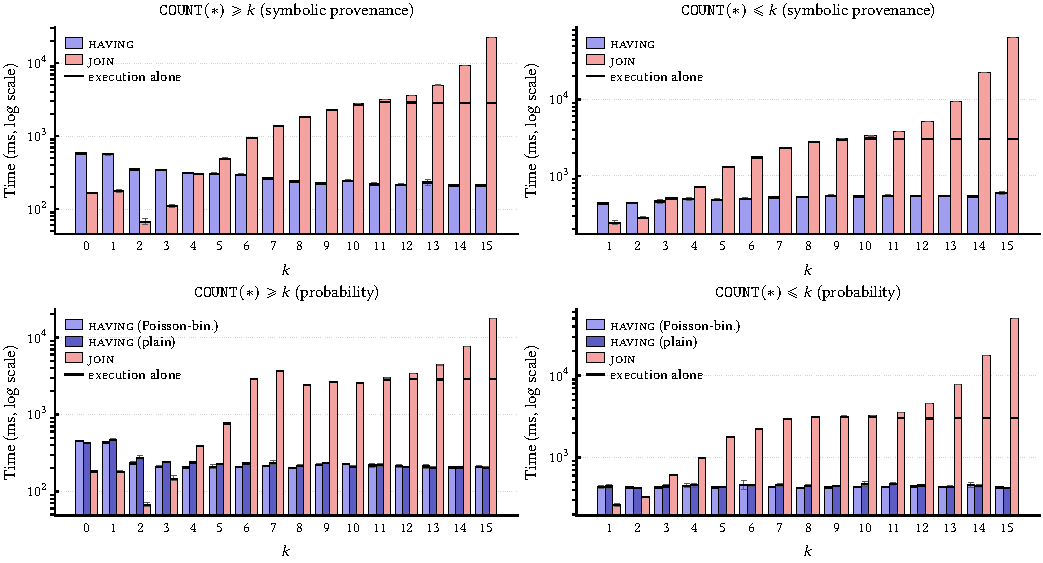
\includegraphics[width=0.9\textwidth]{plots_pierre/bench_fig_combined.pdf}
    \caption{Planning and execution time of the \sql{HAVING} queries
    (\sql{COUNT(*) >= k} on the left, \sql{COUNT(*) <= k} on the right)
    under our semantics and under the self-join rewriting, as a function
    of~$k$: symbolic provenance computation (top) and probability
    evaluation (bottom, with and without the Poisson-binomial optimization
    of Proposition~\ref{prop:agg-cmp-poly-prob}). The height of a bar is
    the planning plus execution time; the black tick marks the execution
    time alone.}
    \label{fig:bench}
\end{figure}

We validate the practical feasibility of this implementation on a
probabilistic image-retrieval database. Following the method
of~\cite{yunus2025using}, the database is built from the objects that
YOLOv5~\cite{ultralytics2021yolov5} detects on the images of a dataset
derived from COCO 2017~\cite{lin2014microsoft}: each detected object is
one tuple of a relation \sql{dataset}, with a unique identifier
\sql{id}, the image identifier \sql{img}, the object class \sql{obj},
and a probability derived from the detector confidence score, treated as
independent probabilistic facts -- $239{,}377$ images and $1{,}570{,}565$
object annotations. We compare, for our possible-world semantics and for
the equivalent self-\sql{JOIN} rewriting (Theorem~\ref{th:correctness})
-- the exact set-up of \cite{yunus2025using}, where the authors had to
use the \sql{JOIN} version as nothing else was available --
(i)~provenance tracking, producing a symbolic provenance formula, and
(ii)~probability computation, for \sql{HAVING} queries with the
comparison \sql{COUNT(*) >= k} or \sql{COUNT(*) <= k}, retrieving the
images with at least (at most) $k$ objects of class 72
(\emph{refrigerator}), $k$ ranging from 0 to 15 (no image has more
than~13).

For probabilistic query evaluation, we use the default ProvSQL pipeline:
a cost-based chooser selects, per provenance circuit, the cheapest exact
method it estimates applicable, from linear-time evaluation of read-once
circuits up to knowledge compilation
(d4~\cite{DBLP:conf/ijcai/LagniezM17}) as a last resort. Here the
circuit of a group has at most 13 inputs, and the \sql{HAVING} queries
are handled by the cheapest methods; the larger circuits of the
\sql{JOIN} rewritings also require tree decompositions and, for some
values of~$k$, knowledge compilation.

For each $k$, every query was executed $3$ times on a desktop computer
(Intel Core i7-12700, 64~GB of RAM) running Ubuntu 22.04, with PostgreSQL
18.6; the figures report the mean of the three runs, with error bars at
one standard deviation, on a logarithmic scale. The height of a bar is
the planning plus execution time measured by \sql{EXPLAIN ANALYZE}, and
a black tick marks the execution time alone. We disabled PostgreSQL's
genetic query optimizer, which by default replaces exhaustive join
ordering from 12 relations onwards: the join orders it selected made the
self-\sql{JOIN} rewritings with $k\geq 12$ exceed a five-minute timeout,
whereas the exhaustive planner keeps their execution around $3$ seconds,
at the price of a planning time that grows quickly with the number of
joins.

Figure~\ref{fig:bench} (top) covers provenance tracking: our semantics
constructs a circuit with a \emph{comparison gate} for the aggregate
comparison, and the possible-world semantics is triggered when
evaluating it in the formula pseudo-semiring (\sql{sr_formula}). As this
pseudo-semiring is not absorptive, the pruning of
Proposition~\ref{prop:algorithms} does not apply, and the valid worlds
of a group are enumerated in full -- at most $2^{13}$ here. The
running time of our semantics is stable as $k$ varies, between $0.2$
and $0.6$ seconds; for \sql{COUNT(*) >= k} it even decreases slowly
with~$k$, as the range check discards more groups. The
\sql{JOIN}-based rewriting is faster for $k\leq 4$, then its cost grows
with the number of joins, up to $14$ times that of our semantics at
$k=11$ and $106$ times at $k=15$, where planning the $15$-way self-join
alone takes $20$ seconds. For \sql{COUNT(*) <= k}, whose rewriting
includes a non-monotone \sql{EXCEPT}, the crossover is at $k=2$, and the
ratio reaches $7$ at $k=11$ and $108$ at $k=15$ ($62$ seconds of
planning for the $16$-way self-join): the stability of our runtime cost
pays off as $k$ increases.

Figure~\ref{fig:bench} (bottom) adds probability evaluation to query
execution and provenance computation.
The \sql{HAVING} semantics, with the Poisson-binomial optimization of
Proposition~\ref{prop:agg-cmp-poly-prob} or without it, stays between
$0.2$ and $0.5$ seconds for all~$k$, the two within a few percent of
each other: with at most $13$ objects per image, the DNF of valid worlds
of a group is small enough for the general pipeline to evaluate by world
enumeration or inclusion--exclusion, so the closed form brings no
measurable gain on this dataset (it would on larger groups, where the
DNF has $\binom{n}{k}$ clauses). The \sql{JOIN} rewriting is cheaper
for~$k\leq 3$, then $12$ to $17$ times slower than our semantics on the
monotone $\geq k$ case and $4$ to $8$ times slower on $\leq k$ up
to~$k=11$, as it pays, on top of the joins, the probability evaluation
of larger circuits, some requiring tree decomposition or knowledge
compilation; beyond, planning dominates and the ratio reaches $83$
and~$115$ at $k=15$. The \sql{JOIN} rewriting is also unable to exploit
the fact that the query becomes vacuously true or false when $k$ exceeds
the number of objects in the images, which both our implementations can.

\begin{toappendix}
  \section{Material for Section~\ref{sec:implementation_experiments}
  (Implementation and Experiments)}
\newcommand{\quotedzero}{\PYG{l+s+s1}{\apos$\mathbb{0}$\apos}}
\label{sec:appendix_impl_experiments}

We present the query templates used for the experiments of
Section~\ref{sec:implementation_experiments}. They are SQL queries using
the functions of the ProvSQL extension of PostgreSQL (\sql{provenance()}, \sql{sr_formula},
\sql{probability_evaluate}, etc.)

The \sql{HAVING}-based template is the following, its condition being
instantiated with \sql{COUNT(*) >= k} or with \sql{COUNT(*) <= k}:
\newcommand{\apos}{\texttt{\textquotesingle}}
\begin{minted}[fontsize=\small, breaklines, escapeinside=||]{postgresql}
SELECT * FROM (
  SELECT img, sr_formula(provenance(), 'image_mapping') AS prov
  FROM dataset
  WHERE obj = c
  GROUP BY img
  HAVING COUNT(*) >= k  -- or:  HAVING COUNT(*) <= k
) sub WHERE prov <> |\quotedzero|;
\end{minted}

For probability evaluation, the call to \sql{sr_formula} in the
projection is replaced by \sql{probability_evaluate(provenance())}, and
the final filter, which
discards the images whose provenance simplifies to~$\mathbb 0$, becomes
\sql{prov > 0}, discarding those whose probability is~$0$; under the
\sql{HAVING} semantics, these are the images for which the aggregate
comparison holds in no possible world.

The equivalent self-\sql{JOIN} rewriting for the ``\sql{>= k}'' case uses
a $(k{-}1)$-fold self-join, with the
``\sql{id > }'' chain ensuring distinct matching tuples:
\begin{minted}[fontsize=\small, breaklines, escapeinside=||]{postgresql}
SELECT * FROM (
  SELECT img, sr_formula(provenance(), 'image_mapping') AS prov
  FROM (
    SELECT DISTINCT d1.img
    FROM dataset d1
    JOIN dataset d2 ON d2.img = d1.img AND d2.obj = c AND d2.id > d1.id
    ...
    JOIN dataset dk ON dk.img = d1.img AND dk.obj = c AND dk.id > d|\(_{k-1}\)|.id
    WHERE d1.obj = c
  ) AS t
) sub WHERE prov <> |\quotedzero|;
\end{minted}

The ``\sql{<= k}'' case is non-monotone and is rewritten as
``at least one match''~\sql{EXCEPT}~``at least~$k+1$ matches'':
\begin{minted}[fontsize=\small, breaklines, escapeinside=||]{postgresql}
SELECT * FROM (
  SELECT img, sr_formula(provenance(), 'image_mapping') AS prov
  FROM (
    SELECT DISTINCT d1.img
    FROM dataset d1
    WHERE d1.obj = c
    EXCEPT
    SELECT DISTINCT d1.img
    FROM dataset d1
    JOIN dataset d2 ON d2.img = d1.img AND d2.obj = c AND d2.id > d1.id
    ...
    JOIN dataset d|\(_{k+1}\)| ON d|\(_{k+1}\)|.img = d1.img AND d|\(_{k+1}\)|.obj = c AND d|\(_{k+1}\)|.id > dk.id
    WHERE d1.obj = c
  ) AS t
) sub WHERE prov <> |\quotedzero|;
\end{minted}
The same projection / zero-filter substitution applies to obtain the
\sql{probability_evaluate} variants of both \sql{JOIN} rewritings.
\end{toappendix}
